% ============================================================
% ch02_architecture.tex
% System Architecture and ER Diagram
% ============================================================

\chapter{System Architecture}

\section{Overview}

The Log-Based Recovery System uses a three-tier architecture:

\begin{enumerate}
  \item \textbf{Data Tier} --- PostgreSQL stores all banking tables
        (Customer, Branch, Account, Transaction\_Record, Employee, Loan).
  \item \textbf{Log Tier} --- MongoDB stores WAL logs, recovery logs,
        and crash event records in three collections.
  \item \textbf{Application Tier} --- Python modules coordinate both
        databases, enforce WAL ordering, and execute recovery.
\end{enumerate}

\begin{figure}[H]
\centering
\begin{tikzpicture}[
  box/.style    = {draw, rounded corners=6pt, minimum width=5.5cm,
                   minimum height=1.1cm, align=center, font=\small},
  dbbox/.style  = {draw, rounded corners=6pt, minimum width=5cm,
                   minimum height=3.8cm, align=center},
  arr/.style    = {-{Latex[length=3mm]}, thick},
  label/.style  = {font=\footnotesize\itshape, align=center},
]

% Application layer
\node[box, fill=green!10, draw=green!60, minimum width=11cm]
  (app) at (0, 4.5) {\textbf{Python Application Layer}\\
  \small main.py \quad transaction\_manager.py \quad recovery\_manager.py};

% PostgreSQL box
\node[dbbox, fill=blue!8, draw=blue!50] (pg) at (-3.2, 1.5) {
  \textbf{PostgreSQL}\\[6pt]
  \footnotesize Customer\\
  \footnotesize Branch\\
  \footnotesize Account\\
  \footnotesize Transaction\_Record\\
  \footnotesize Employee, Loan
};

% MongoDB box
\node[dbbox, fill=orange!8, draw=orange!50] (mg) at (3.2, 1.5) {
  \textbf{MongoDB}\\[6pt]
  \footnotesize wal\_logs\\
  \footnotesize recovery\_logs\\
  \footnotesize crash\_log\\
  \footnotesize system\_config
};

% Arrows
\draw[arr] (app.south) -- ++(0,-0.4) -| (pg.north)
  node[pos=0.3, above, label] {ACID transactions\\psycopg2};
\draw[arr] (app.south) -- ++(0,-0.4) -| (mg.north)
  node[pos=0.3, above, label] {WAL logs\\pymongo};

% WAL arrow
\draw[arr, dashed, color=red!70, very thick]
  (mg.south) -- ++(0,-0.6) -| (pg.south)
  node[midway, below, font=\footnotesize\bfseries\color{red!70}]
  {Recovery Manager reads logs → fixes PostgreSQL};

\end{tikzpicture}
\caption{System Architecture: Python coordinates PostgreSQL and MongoDB}
\label{fig:architecture}
\end{figure}

\section{Component Roles}

\subsection{PostgreSQL --- Data Store}
PostgreSQL serves as the ground truth for banking data. It holds:
\begin{itemize}
  \item Current account balances (the data being protected)
  \item Transaction history records
  \item Customer, Branch, Employee, and Loan information
\end{itemize}
PostgreSQL transactions are controlled manually with explicit
\texttt{conn.commit()} and \texttt{conn.rollback()} calls.

\subsection{MongoDB --- WAL Log Store}
MongoDB stores Write-Ahead Log documents. Each document captures:
\begin{itemize}
  \item The \textit{old\_balance} before the change (used for UNDO)
  \item The \textit{new\_balance} after the change (used for REDO)
  \item The transaction status: \texttt{UNCOMMITTED}, \texttt{COMMITTED},
        or \texttt{ROLLED\_BACK}
\end{itemize}
MongoDB is used independently of the PostgreSQL transaction --- a failed
PG transaction does not affect the MongoDB log entry.

\subsection{Python Recovery Module}
Five Python modules coordinate the system:

\begin{table}[H]
\centering
\caption{Python Module Responsibilities}
\begin{tabularx}{\textwidth}{llX}
\toprule
\textbf{File} & \textbf{Class} & \textbf{Responsibility} \\
\midrule
db\_config.py & --- & PostgreSQL and MongoDB connection functions \\
mongo\_logger.py & MongoLogger & WAL log writes, updates, queries \\
transaction\_manager.py & TransactionManager & Deposit, withdraw, transfer with WAL \\
crash\_simulator.py & CrashSimulator & Mid-transaction crash injection \\
recovery\_manager.py & RecoveryManager & UNDO + REDO + Analysis phases \\
main.py & --- & Interactive menu-driven demo interface \\
\bottomrule
\end{tabularx}
\end{table}

\section{WAL Data Flow}

\begin{figure}[H]
\centering
\begin{tikzpicture}[
  step/.style = {draw, rounded corners=4pt, fill=gray!10,
                 minimum width=10cm, minimum height=0.8cm,
                 align=center, font=\small},
  crash/.style = {draw, rounded corners=4pt, fill=red!15, draw=red!60,
                  minimum width=10cm, minimum height=0.8cm,
                  align=center, font=\small\bfseries},
  arr/.style  = {-{Latex[length=3mm]}, thick},
]
\node[step]   (s1) at (0, 6)    {1. Read old\_balance from PostgreSQL};
\node[step, fill=yellow!20, draw=orange!70] (s2) at (0, 4.8)
  {\textbf{2. Write WAL log to MongoDB (status = UNCOMMITTED)} $\leftarrow$ WAL written FIRST};
\node[step]   (s3) at (0, 3.6)  {3. Update Account balance in PostgreSQL};
\node[step]   (s4) at (0, 2.4)  {4. Insert Transaction\_Record in PostgreSQL};
\node[step]   (s5) at (0, 1.2)  {5. conn.commit() --- PostgreSQL COMMIT};
\node[step, fill=green!15, draw=green!60]
              (s6) at (0, 0)    {6. Update MongoDB WAL log (status = COMMITTED)};
\node[crash]  (cx) at (6.5, 2.8) {$\Uparrow$ CRASH here\\leaves log UNCOMMITTED};

\draw[arr] (s1)--(s2); \draw[arr] (s2)--(s3);
\draw[arr] (s3)--(s4); \draw[arr] (s4)--(s5); \draw[arr] (s5)--(s6);
\draw[->, dashed, red!70, thick] (cx.west) -- (s3.east);
\end{tikzpicture}
\caption{WAL Transaction Sequence --- 6 steps}
\label{fig:wal_flow}
\end{figure}

% ────────────────────────────────────────────────────────────
\chapter{Entity-Relationship Diagram}

\section{ER Diagram Overview}

The database schema consists of six entities with the following relationships:

\begin{figure}[H]
\centering
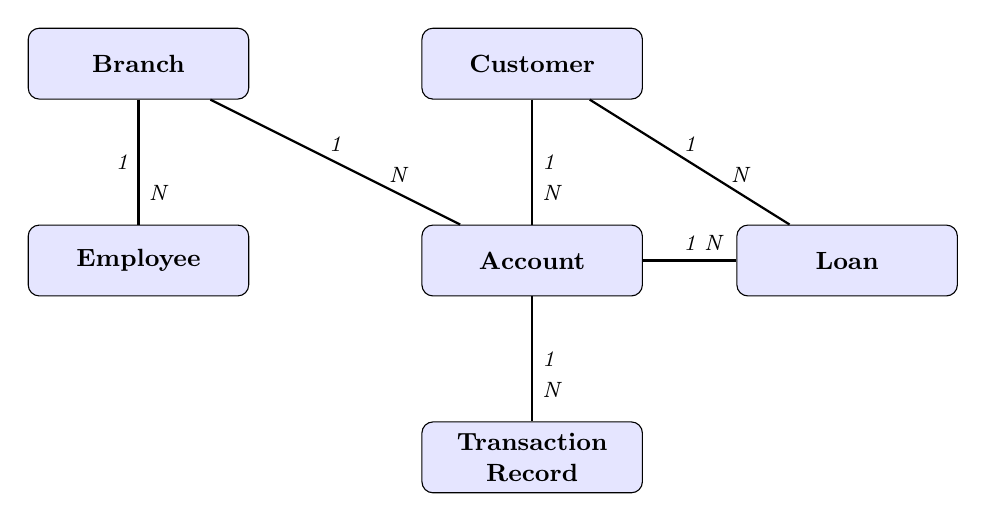
\begin{tikzpicture}[
  entity/.style = {draw, rectangle, rounded corners=4pt,
                   fill=blue!10, minimum width=2.8cm,
                   minimum height=0.9cm, align=center, font=\small\bfseries},
  rel/.style    = {font=\footnotesize\itshape},
  arr/.style    = {thick},
]
% Entities
\node[entity] (branch)   at (0, 6)    {Branch};
\node[entity] (customer) at (5, 6)    {Customer};
\node[entity] (employee) at (0, 3.5)  {Employee};
\node[entity] (account)  at (5, 3.5)  {Account};
\node[entity] (txn)      at (5, 1)    {Transaction\\Record};
\node[entity] (loan)     at (9, 3.5)  {Loan};

% Relationships
\draw[arr] (branch)   -- node[rel, left]  {1}  (employee)
           node[rel, right, near end] {N} {};
\draw[arr] (branch)   -- node[rel, above] {1}  (account)
           node[rel, above, near end] {N} {};
\draw[arr] (customer) -- node[rel, right] {1}  (account)
           node[rel, right, near end] {N} {};
\draw[arr] (account)  -- node[rel, right] {1}  (txn)
           node[rel, right, near end] {N} {};
\draw[arr] (customer) -- node[rel, above] {1}  (loan)
           node[rel, above, near end] {N} {};
\draw[arr] (account)  -- node[rel, above] {1}  (loan)
           node[rel, above, near end] {N} {};
\end{tikzpicture}
\caption{Entity-Relationship Diagram}
\label{fig:er}
\end{figure}

\section{Relationships and Cardinality}

\begin{table}[H]
\centering
\caption{Entity Relationships}
\begin{tabularx}{\textwidth}{llX}
\toprule
\textbf{Entity 1} & \textbf{Entity 2} & \textbf{Relationship} \\
\midrule
Branch   & Employee           & One branch employs many employees (1:N) \\
Branch   & Account            & One branch hosts many accounts (1:N) \\
Customer & Account            & One customer can have many accounts (1:N) \\
Account  & Transaction\_Record & One account has many transactions (1:N) \\
Customer & Loan               & One customer can have many loans (1:N) \\
Account  & Loan               & One account linked to many loans (1:N) \\
\bottomrule
\end{tabularx}
\end{table}

\section{Normalization}

The schema is normalized to \textbf{Third Normal Form (3NF)}:

\begin{itemize}
  \item \textbf{1NF}: All attributes are atomic. No multi-valued fields.
  \item \textbf{2NF}: No partial dependencies. All non-key attributes depend
        fully on the primary key.
  \item \textbf{3NF}: No transitive dependencies. Branch information is stored
        in the Branch table, not repeated in Account or Employee.
\end{itemize}
